\subsection{Voxelization}\paragraph{}
Normally a volume is populated using some accompanying static 3D texture data. For our implementation we manually update out voxel individually. 

We want our final voxels to represent the billowing, semi-spherical shape of a cloud. We also want to  highlight the voxels nearest to the light source which will be essential when shading the cloud. 

To voxelize we clear the entire volume on every frame and rerun our full voxelization algorithm. This will be necessary if we ever add procedurally animated clouds. 

\subsubsection{Spherical Billboards}\paragraph{}
We begin by rendering many billboards from the light's perspective. In the fragment shader we calculate a spherical distribution mapped to the face of the billboard. Using this distribution we populate a sphere within the volume. 

% Code defining inital spherical voxelization
\begin{lstlisting}[caption={first\_voxelize.glsl, 42}]
// Calculate tthe distance from the center of the billboard to the current fragment
float fragDist = distance(center, fragPos);
// Calculate a linear distribution [0, 1]
float distribution = fragDist / radius;
// Convert the linear distribution to spherical [0, 1]
distribution = sqrt(max(0, 1 - distribution * distribution));
// Calculate the near point of the sphere intersecting this fragment
float sphereDistance = radius * distribution;
vec3 nearPos = fragPos + billboardNormal * sphereDistance;
// Iterate from the front of the sphere to back 
// Set the voxels within this line to black
for(float scale = 0; scale < 2 * sphereDistance; scale += stepSize) {
	vec3 worldPos = nearPos - billboardNormal * scale;
	imageStore(volume, getVoxelIndex(worldPos), vec4(0,0,0,1));
}
\end{lstlisting}\paragraph{}

% first voxelization pass figures
\begin{figure}[t]
\centering
	\begin{subfigure}[t]{0.48\textwidth}
	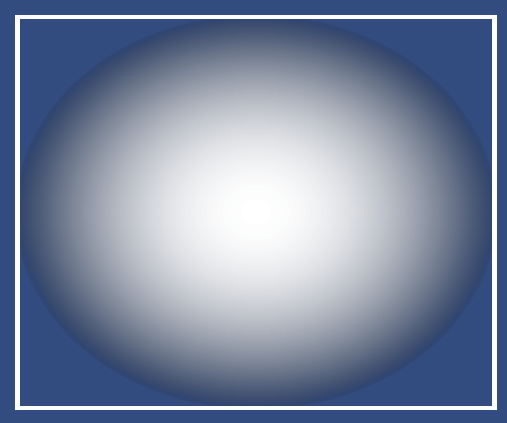
\includegraphics[width=\textwidth]{../res/spherebillboard.png}
	\caption{Spherical distribution mapped to a billboard}
	\end{subfigure}
	~
	\begin{subfigure}[t]{0.48\textwidth}
	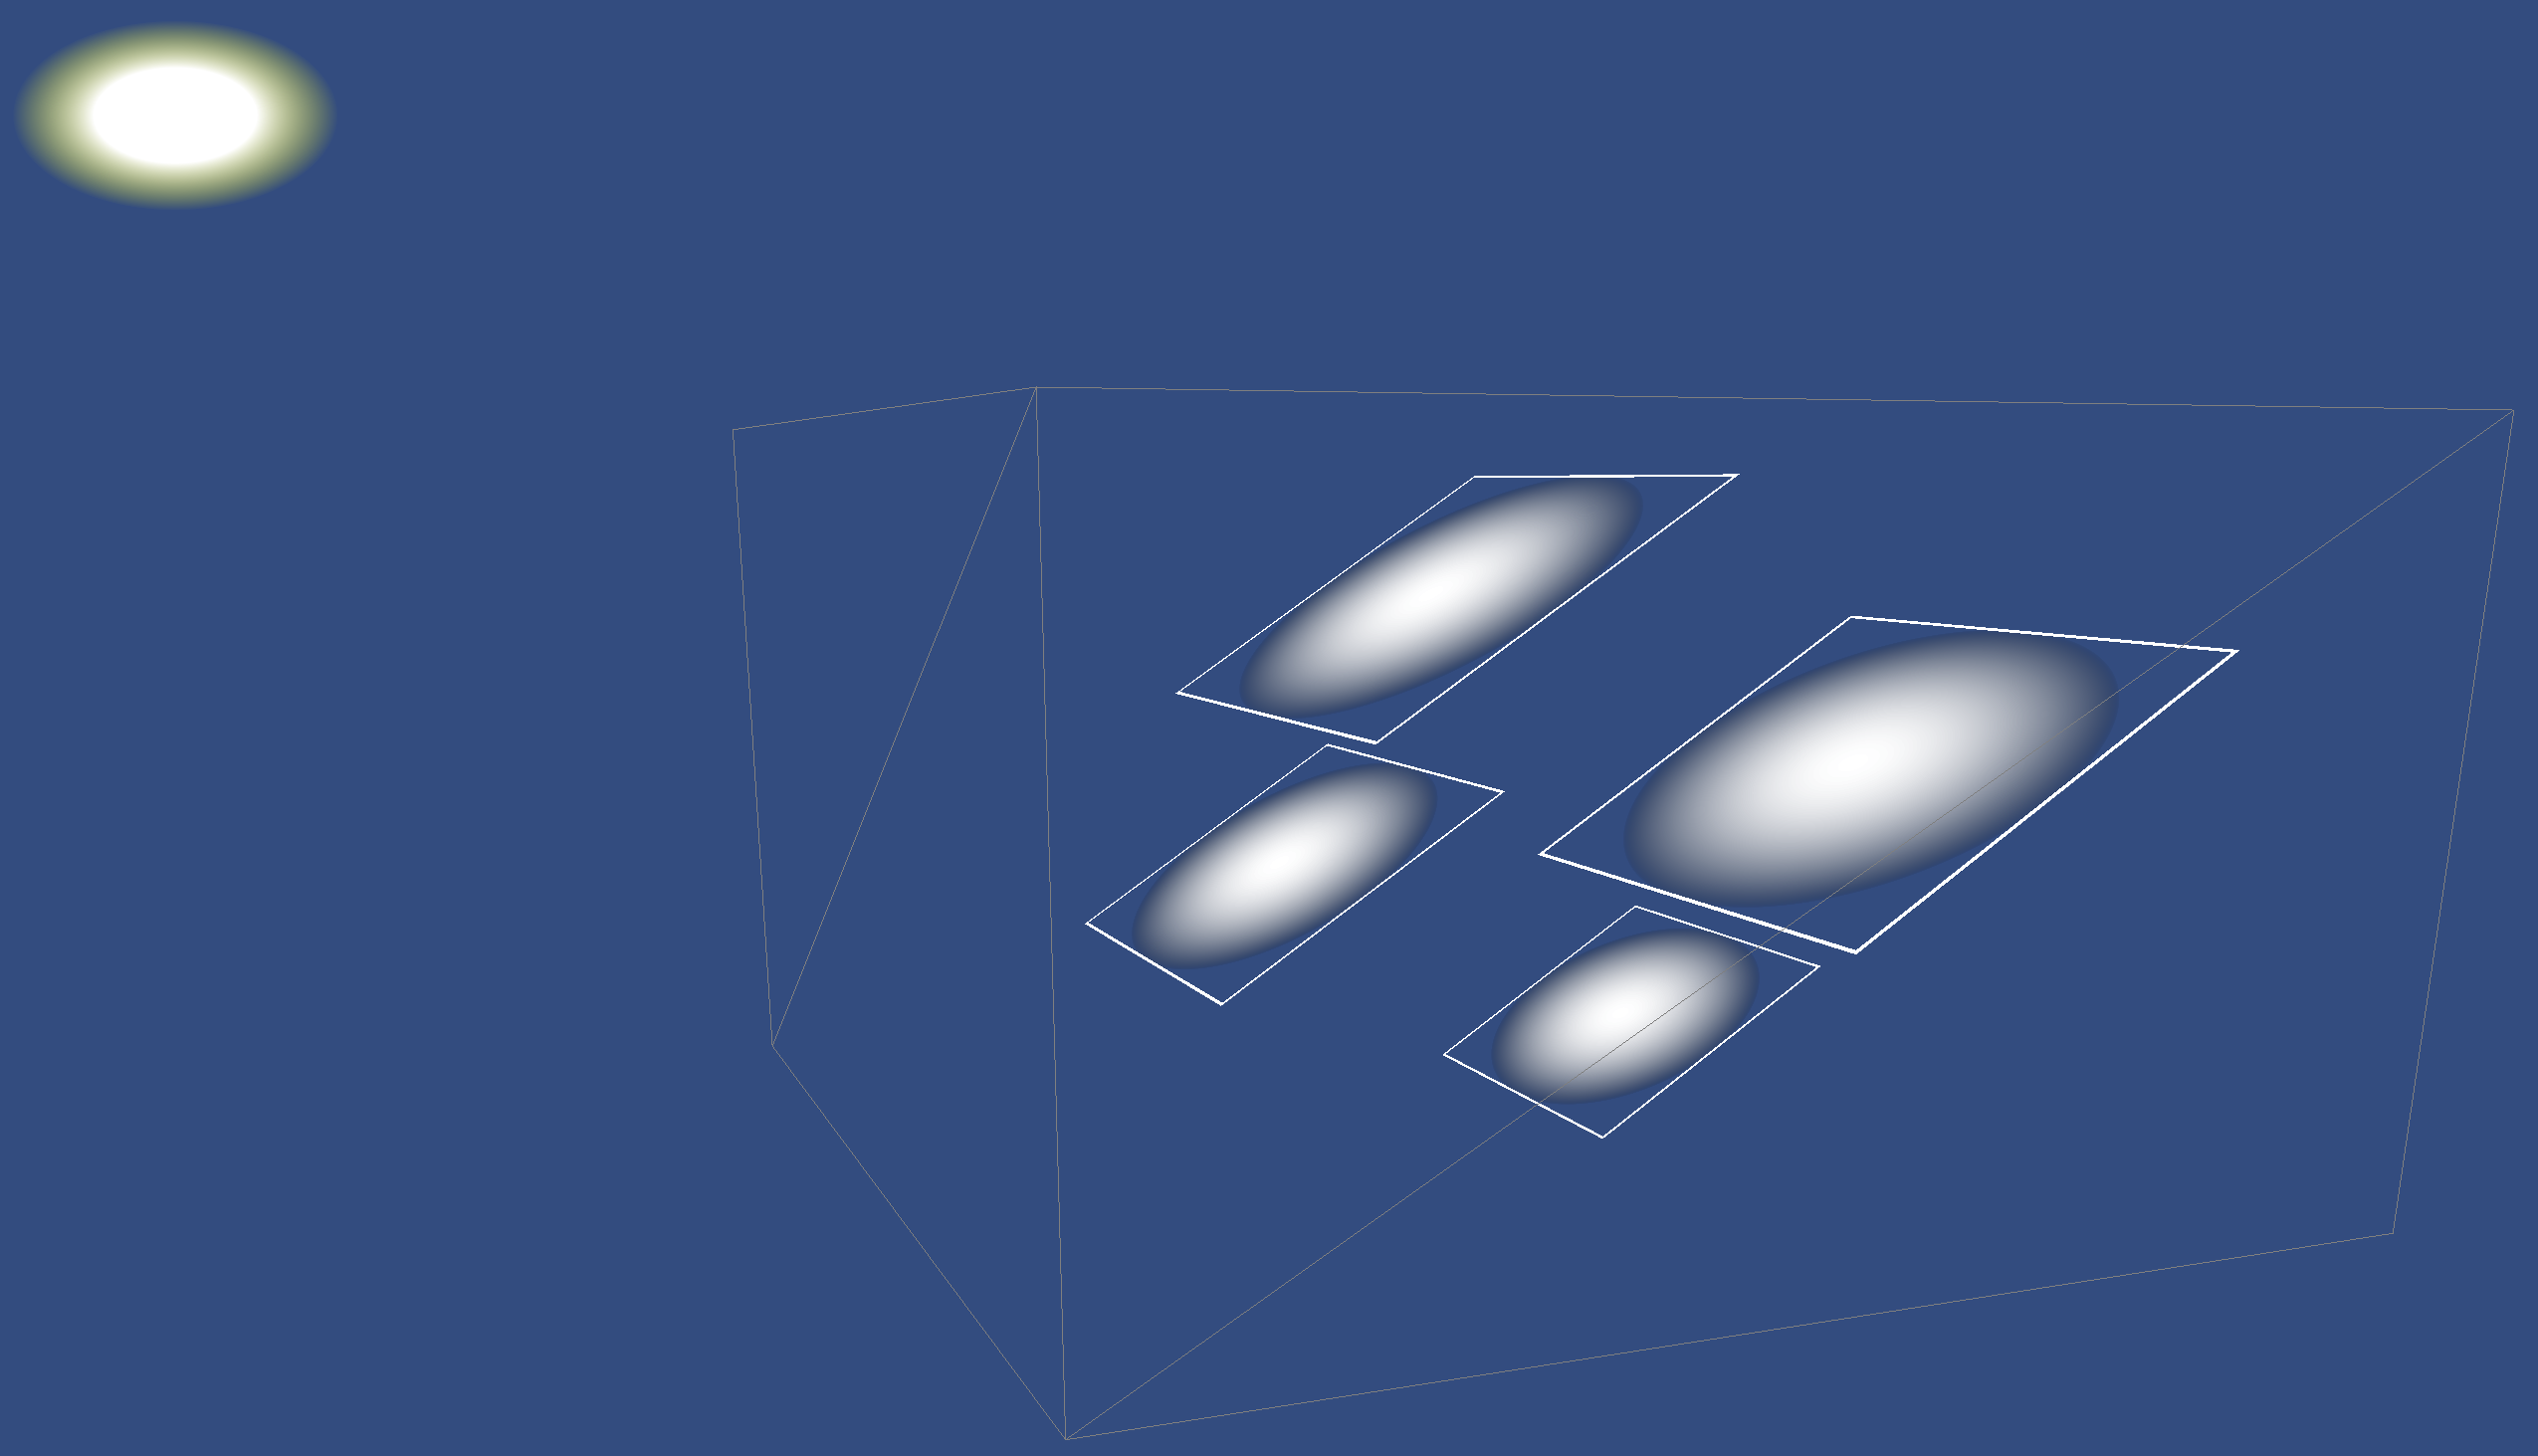
\includegraphics[width=\textwidth]{../res/lightfacing.png}
	\caption{Light-facing billboards}
	\end{subfigure}
	~
	% TODO : diagram
	% TODO : should this be its own figure?
	\begin{subfigure}[t]{0.48\textwidth}
	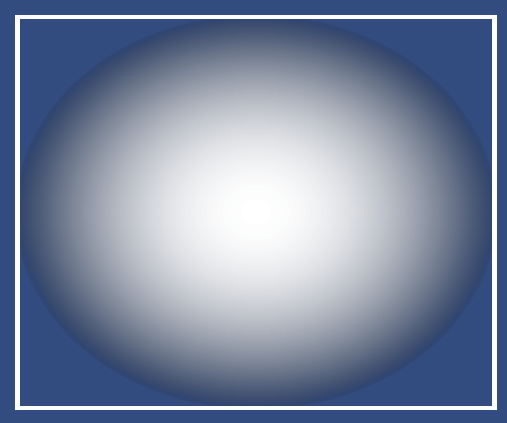
\includegraphics[width=\textwidth]{../res/spherebillboard.png}
	\caption{Diagram of first-voxelization pass}
	\end{subfigure}
	~
	\begin{subfigure}[t]{0.48\textwidth}
	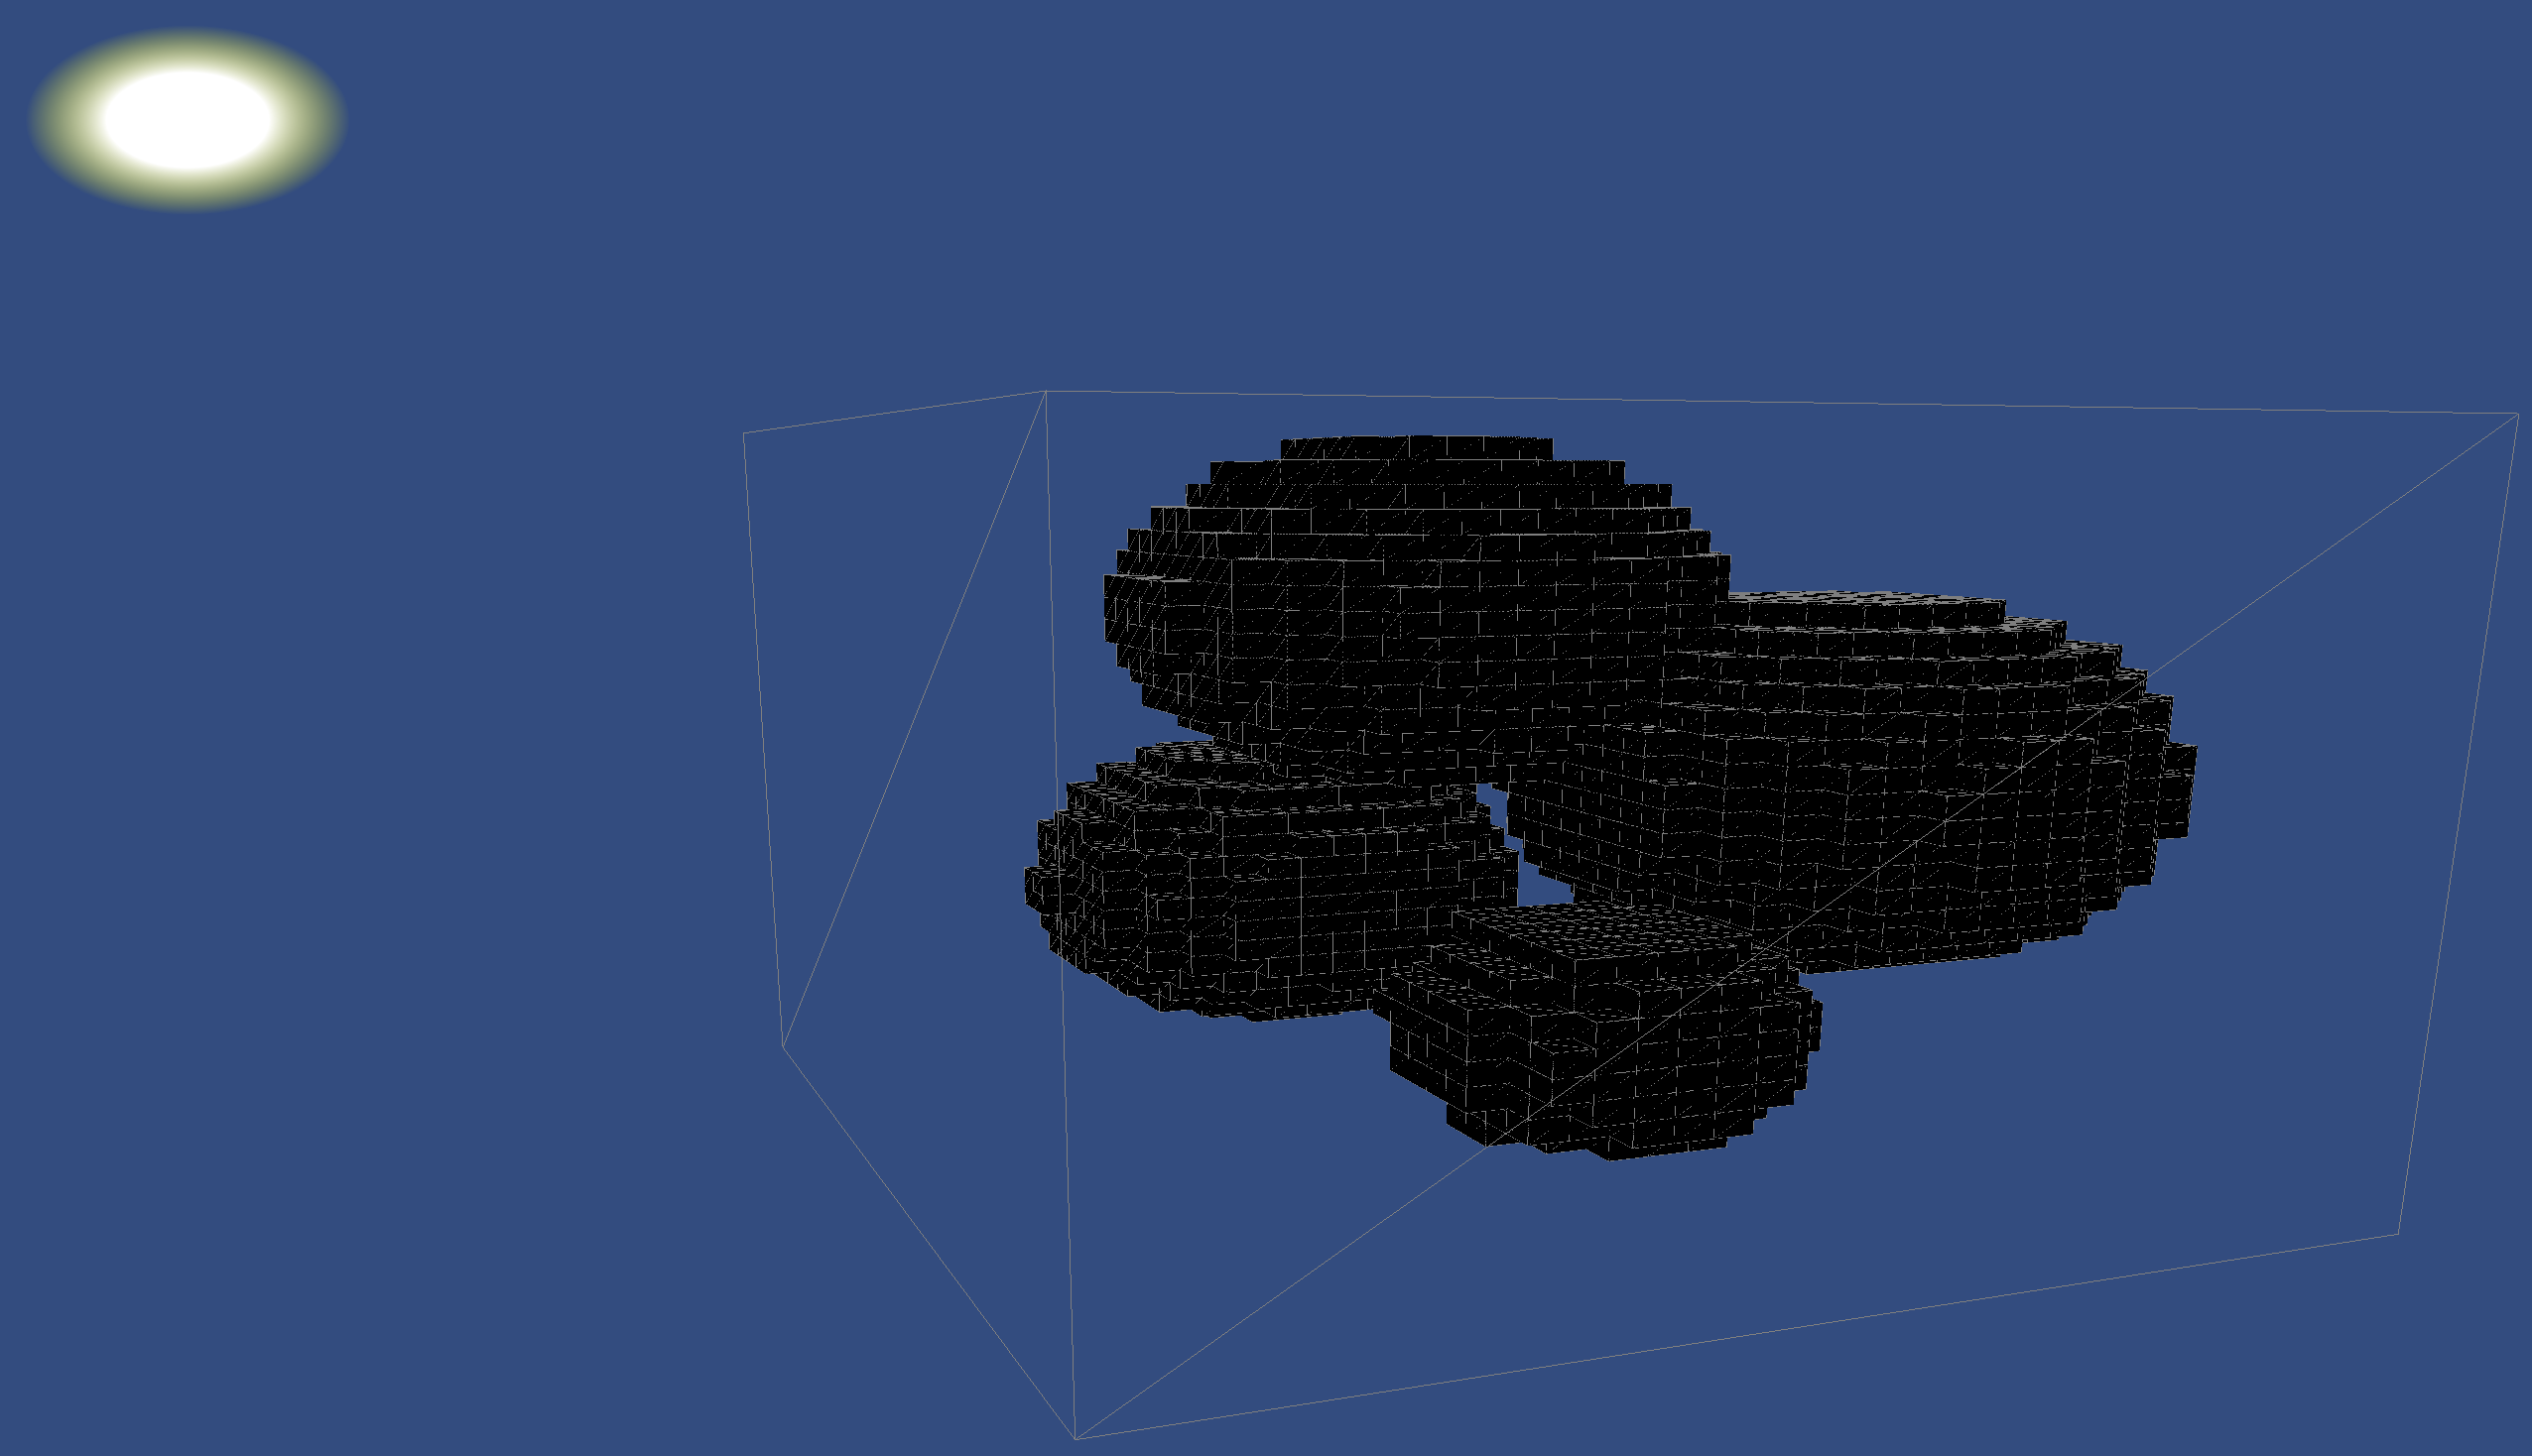
\includegraphics[width=\textwidth]{../res/voxelize1.png}
	\caption{Voxelization of spherical billboards}
	\end{subfigure}
\caption{First voxelization pass of 4 billboards}
\end{figure}

\newpage
\subsubsection{Position Map}\paragraph{}
We could have rendered these billboard from the camera's perspective and achieved the same voxelization results. We chose to render from the light's perspective because we want to keep track of which voxels are nearest to the light source. 
During our first voxelization pass we write out the sphere's positions to the frame buffer being rendered to. This frame buffer, once all billboards have been rendered, will contain the world positions of the voxels nearest to the light source. 

This method utilizes the graphics pipeline's depth test to occlude spheres any sphere that is hidden by nearer spheres.
The depth test, however, relies on rasterized geometry in the z-buffer, and the geometry being rendered is the flat billboards, not the spherical distributions that they represent! To solve this we manually calculate and write the sphere's depth into the z-buffer. We do this in world-space using the light perspective's near and far plane. It would likely be more elegant and efficient to do this calculation in clip-space.
% Calculating and writing to position map
\begin{lstlisting}[caption={first\_voxelize.glsl, 60}]
// Calculate sphere fragment's world position 
// This is the position nearest to the light source at this fragment
vec3 nearPos = fragPos + billboardNormal * sphereDistance;
// Calculate sphere fragment's depth within the light's perspective
float viewSize = distance(lightNearPlane, lightFarPlane);
float depth = distance(lightNearPlane, nearPos) / viewSize;
// Write position and depth to frame buffer
outColor = vec4(nearPos, 1);
gl_FragDepth = depth;
\end{lstlisting}

% Position map
\begin{figure}[h]
\centering
	% color attachment
	\begin{subfigure}[t]{0.48\textwidth}
	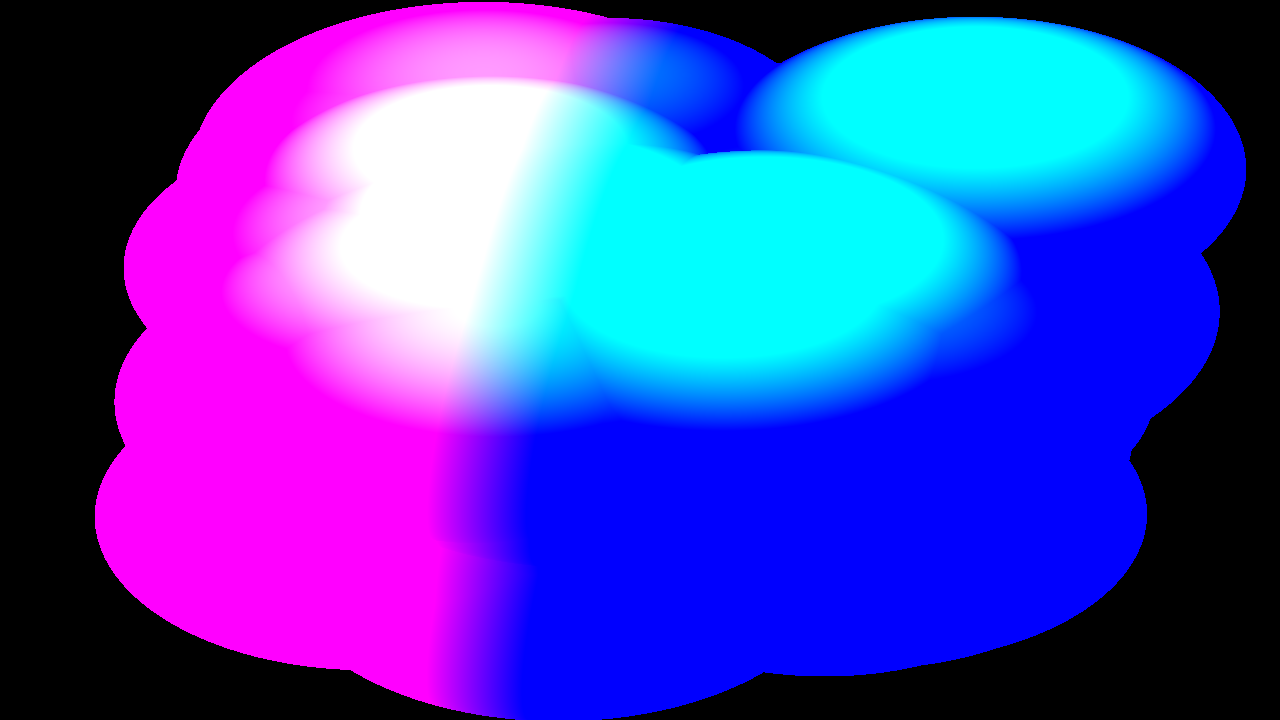
\includegraphics[width=\textwidth]{../res/positionmapcolor.png}
	\caption{Color attachment}
	\end{subfigure}
	~
	% depth attachment 
	\begin{subfigure}[t]{0.48\textwidth}
	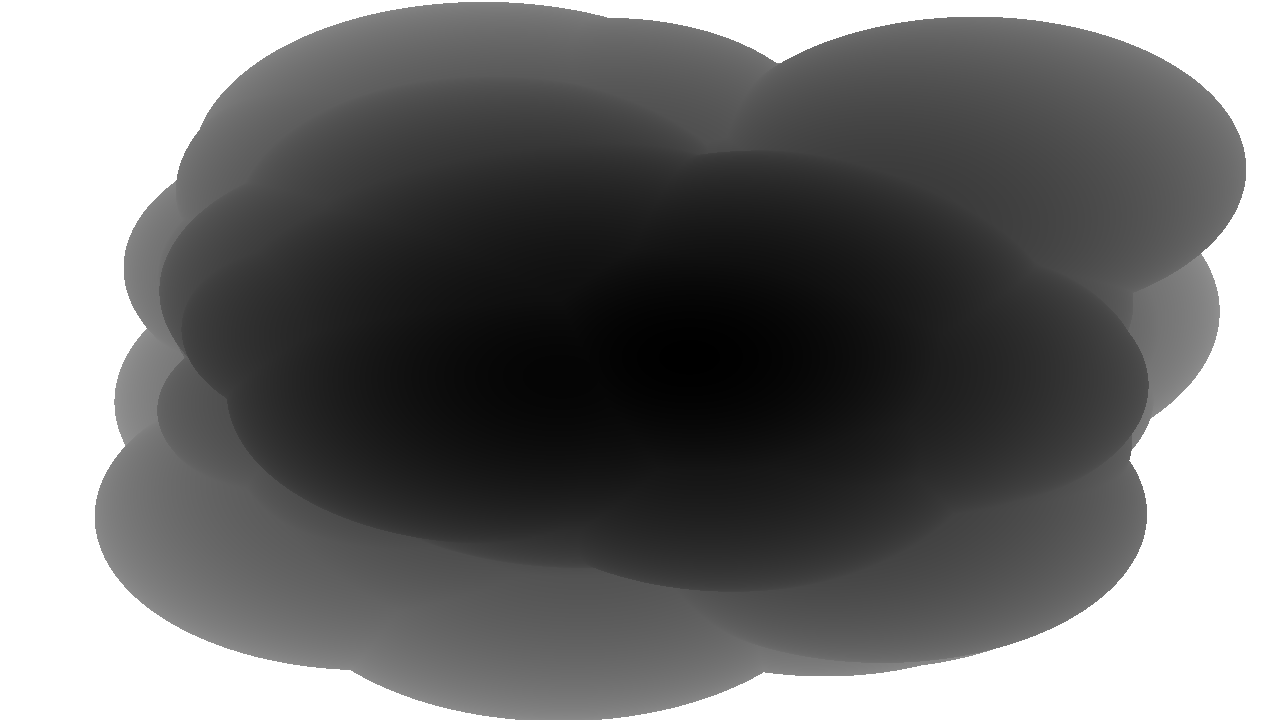
\includegraphics[width=\textwidth]{../res/positionmapdepth.png}
	\caption{Depth attachment}
	\end{subfigure}
\caption{Final position map after first pass}
\end{figure}

The final result of the position map is a screen-sized texture containing the world positions of voxels nearest to the camera. This data can be used to highlight those voxels.

\subsubsection{Highlighting voxels}\paragraph{}
For our second voxelization pass we render position map to the screen on a full-sized quad. 
We sample each fragment of the position map to get the world positions of voxels nearest to the light source, and we then update the voxel at that world position to highlight that it is on the outer layer of the cloud. 

% second voxelize
\begin{lstlisting}[caption={second\_voxelize.glsl, 34}]
// Get world position of voxels from position map
vec4 worldPos = imageLoad(positionMap, ivec2(gl_FragCoord.xy));
// Only highlight the voxel if the position map sample is valid
if (worldPos.a >= 0.f) {
    imageStore(volume, calculateVoxelIndex(worldPos.xyz), vec4(1));
}
\end{lstlisting}

%

The final result of our voxelization algorithm is a billowing spherical cloud-like structure with the voxels nearest to the camera being highlighted. 

\begin{figure}[h]
\centering
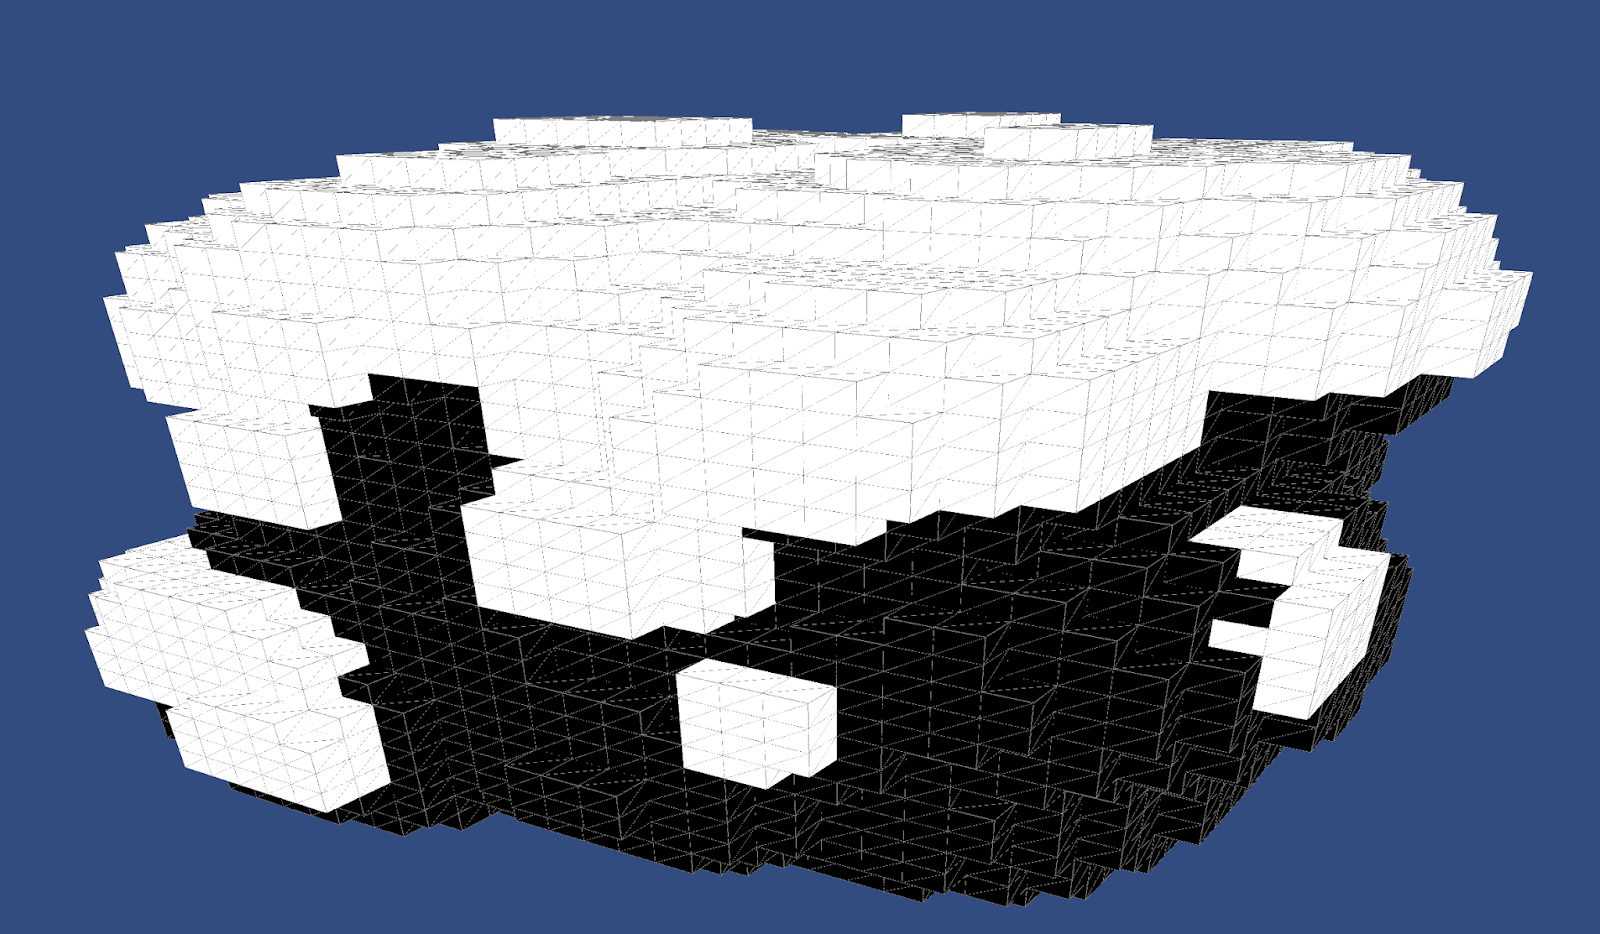
\includegraphics[width=\textwidth]{../res/billowing.png}
\caption{Final result of voxelization}
\end{figure}

% TODO : \subsubsection{Optimizations}
% TODO : light view
% TODO : rg 8?
% TODO : no need for first voxelization pass
% TODO : concurrency
